\documentclass[30pt, a0paper, portrait, margin=0mm, innermargin=15mm,
               blockverticalspace=15mm, colspace=15mm, subcolspace=8mm]{tikzposter} 

% Change font     
\renewcommand{\familydefault}{\sfdefault}

\definecolor{mycol}{HTML}{326E77}
\definecolorstyle{myColorStyle}{
  \colorlet{colorOne}{darkgray}
  \colorlet{colorTwo}{gray}
  \colorlet{colorThree}{gray}
}{
  % Background Colors
  \colorlet{backgroundcolor}{colorTwo!50}
  \colorlet{framecolor}{black}
  % Title Colors
  \colorlet{titlefgcolor}{black}
  \colorlet{titlebgcolor}{colorOne}
  % Block Colors
  \colorlet{blocktitlebgcolor}{mycol}
  \colorlet{blocktitlefgcolor}{white}
  \colorlet{blockbodybgcolor}{white}
  \colorlet{blockbodyfgcolor}{black}
  % Innerblock Colors
  \colorlet{innerblocktitlebgcolor}{white}
  \colorlet{innerblocktitlefgcolor}{black}
  \colorlet{innerblockbodybgcolor}{white}
  \colorlet{innerblockbodyfgcolor}{black}
  % Note colors
  \colorlet{notefgcolor}{black}
  \colorlet{notebgcolor}{white}
  \colorlet{notefrcolor}{white}
}

% LATEX PACKAGES
% --------------
  
\usepackage{graphicx}  % package for inserting images, including .pdf
\usepackage{adjustbox} % package for cropping images
\usepackage[colorlinks=true, urlcolor=red]{hyperref} % package for url and hyperlinks
\usepackage{wrapfig}
\usepackage{lmodern} %mix italic and bold
\usepackage{hyperref}% for url
\usepackage{authblk}
\usepackage{graphicx} 
\usepackage{caption}
\usepackage{mwe}
\usepackage[absolute]{textpos}


% TITLE, AUTHORS, INSTITUTE
% -------------------------

\title{\textbf{Co-evolution of house mouse and an intracellular parasite, \textit{Eimeria} spp.}}
\author[1,2]{Alice~Balard}
\author[1,2]{Victor~Jarquin}
\author[1]{Francisca~B\"ohning}
\author[1]{Thi~Phuong~Li}
\author[3]{Stuart~J.E.~Baird}
\author[3]{Jaroslav~Pi\`alek}
\author[4]{D.T?}
\author[1,2]{Emanuel~Heitlinger}
\affil[1]{\Large Ecology and Evolution of molecular Parasite-Host Interactions (HU/IZW), Leibniz Institute for Zoo and Wildlife Research (IZW) in the Forschungsverbund Berlin e.V. Alfred-Kowalke-Strasse 17, 10315 Berlin, Germany}
\affil[2]{\Large Department of Molecular Parasitology, Humboldt University, Philippstrasse 13, 10115 Berlin, Germany}
\affil[3]{\Large Department of Population Biology, Institute of Vertebrate Biology, ASCR, Brno and Studenec, Czech Republic\vspace{-6ex}% reduce space
}

\makeatletter
\def\maketitle{\AB@maketitle}
\makeatother

% THEME SETTING
% -------------
\usetheme{Default}
\usecolorstyle{myColorStyle}
\useblockstyle{Basic}
\usebackgroundstyle{Empty}
\usetitlestyle{Empty}


% HEAD
% ----

\begin{document}
\maketitle
\begin{columns}

% ------------------------
% COLUMN 1 ---------------

\column{0.5}

% Context
% ----

\block{Context}
{
	\begin{itemize}
		\item House Mouse Hybrid Zone, 20km wide, formed by hybrids of \textit{Mus musculus domesticus} and \textit{Mus musculus musculus}. After 500,000 years in isolation, secondary contact 5000 years ago (Machol\'{a}n \textit{et al.} 2012; Boursot \textit{et al.} 1993)

        \begin{center}
          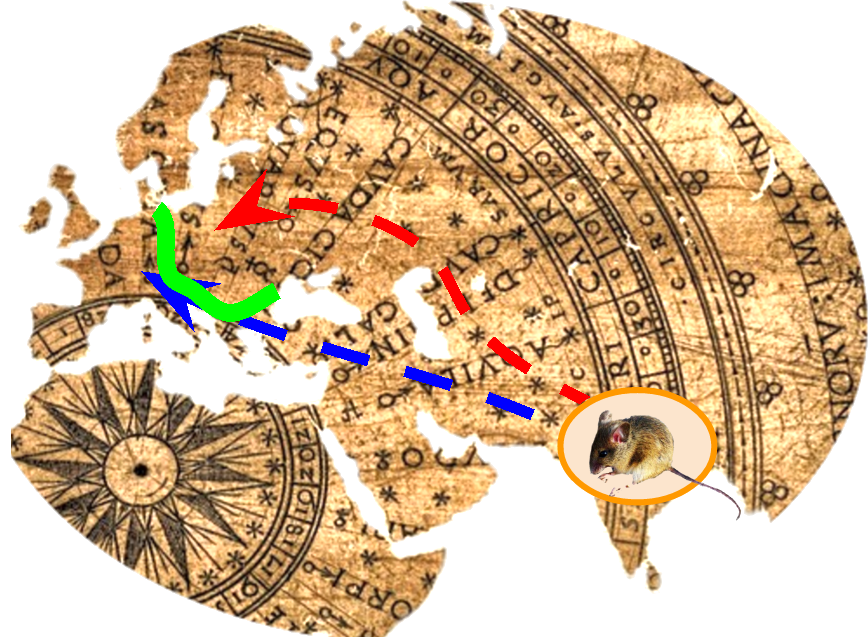
\includegraphics[scale=0.8]{R7.png}
        \end{center}
        		\item Eimeria spp., obligate intracellular apicomplexan parasite. \textbf{Two major clades (A \& B)} of \textit{Eimeria} spp. identified (3 markers) in the mice of the hybrid zone (Jost 2016)
        \end{itemize}
}

% AIMS
% ----

\block{Aims of the study}
{
	\begin{enumerate}
	\item Investigating the \textbf{ vigor/resistance of hybrids of house mouse} to their parasite\\ \textit{Eimeria}~spp. using prevalence and intensity data for parasite strains throughout the\\ House Mouse Hybrid Zone.
	\item Looking for evidence of \textbf{local adaptation} between the murine host and its Eimerian parasite
	\end{enumerate}
}


% Material \& Methods : Field study
% -------
\block{Material \& Methods : Field study}
{     \begin{itemize}

       \item{Annual sampling every September\\ 104 mice in 2015 from 48 localities\\ 103 mice in 2016 from 34 localities \\ upcoming sampling in 2017 \\ Brandenburg area (Germany)}
       \item{Oocyst counted in mice feces\\ All parasite strains genotyped using 3 markers, then assigned to an \\haplotype}
     
      \item Adaptation of the method of Stuart J.E. Baird (Baird \textit{et al.} 2012) : Maximum likelihood analysis explicitly linking parasite abundance to a gradient along the hybrid index (as a proxy of host heterozygosity), generalized linear model with negative binomial distribution \vspace{+1ex}
      \textcolor{blue}{\[Parasite\ load \sim mouse\ heterozygosity\ level * parasite\ strain  \]}\vspace{-2ex}% reduce space
      \item R package under development : \url{https://github.com/alicebalard/Parasite_Load}
      \end{itemize}
      }

% Material \& Methods : Cross infection
% -------

\block{Material \& Methods : Cross infection}
      {Pilote experiment
      \begin{itemize}
      
      \item Parasite strains :
      
      \begin{enumerate}
      \item \textbf{\textit{Eimeria} haplotype A} laboratory strain \textit{Eimeria falciformis} REEEFF
      \item \textbf{\textit{Eimeria} haplotype B} strain isolated in the wild 
      \end{enumerate}
      
      \item Host strains :
      
      \begin{enumerate}
      \item \textbf{WSB} Wild-derived inbred strain. Isolated from wild \textit{Mus musculus domesticus}\\ Region of capture : Eastern Shore, Maryland
      \item \textbf{PWD} Wild-derived inbred strain. Isolated from wild \textit{Mus musculus musculus}\\ Region of capture : near Prague, Czech Republic
      \item \textbf{WP} Hybrids between the 2 previous commercial strains
      \end{enumerate}
      
      \end{itemize}
}


      % ACKNOWLEDGEMENTS
% ----------------
      \note[targetoffsetx=-15cm, targetoffsety=-13cm, width=25cm, innersep=0cm]
{
    \begin{wrapfigure}{r}{2cm}	
   \vspace{-55pt}
   
	
\includegraphics[scale=0.41]{Logos.png}
	
	\end{wrapfigure}
	\textbf{Funding :} This research has received funding 
	from the DFG, and is part of a IZW/HU project\\
        A. Balard is part of the Dahlem Research School\\
        \textbf{Contact :} \textcolor{blue}{alice.balard@fu-berlin.de}
}


% ------------------------
% COLUMN 2 ---------------

\column{0.5}


\block{Preliminary results : exploring hybrid vigor/resistance in the wild}
{

\vfill
\begin{minipage}{0.3\linewidth}
    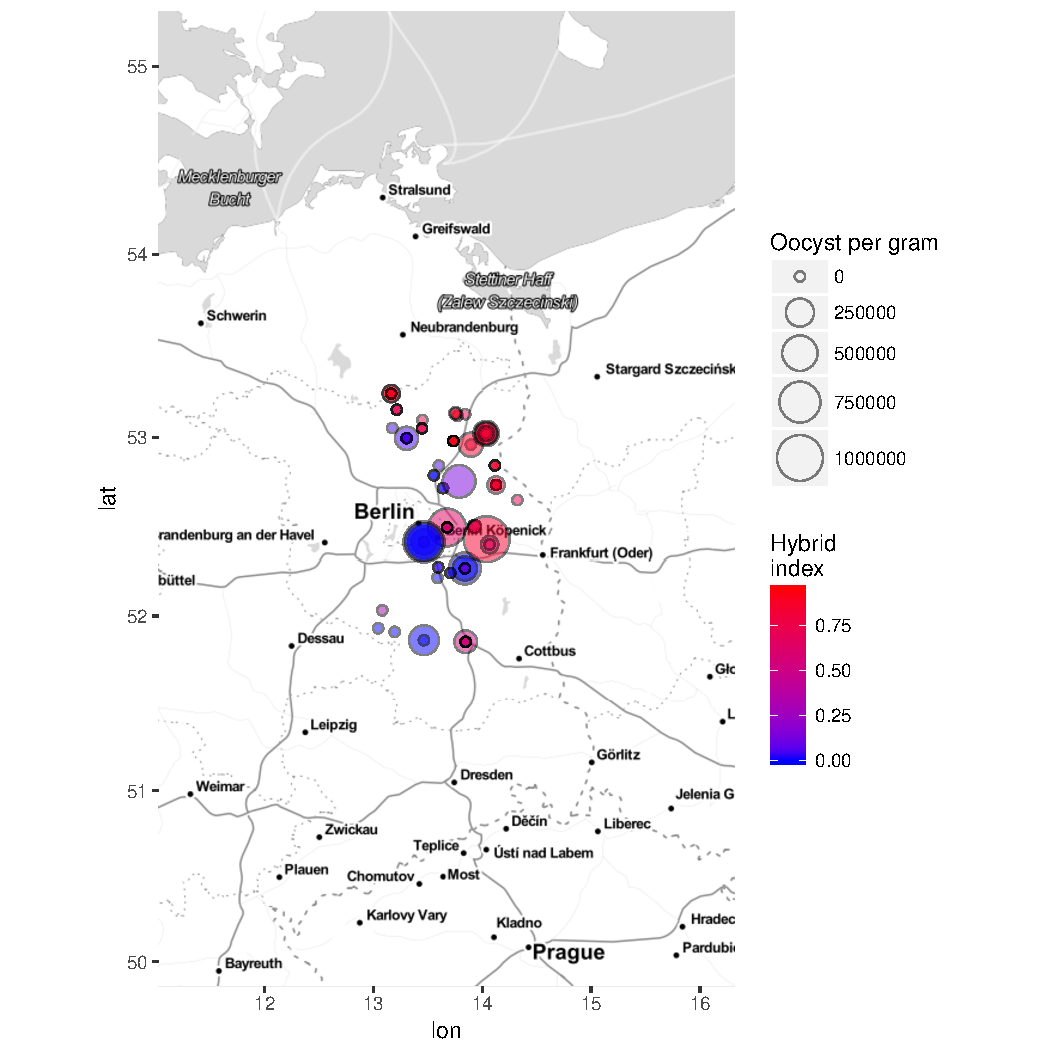
\includegraphics[width=2\linewidth]{Map2015-2016_temp.pdf}
\end{minipage}
%\hfil
\hspace{11cm}
\begin{minipage}{0.4\linewidth}
 \begin{itemize}
      \item{Prevalence : \\19\% infected farms in 2015\\ 2016 : pending analysis... \\ 2017 : upcoming sampling}\\
       \item{Hybrid index assigned to all mice \\0 = \textit{\textcolor{blue}{Mus musculus domesticus}}\\
       1 = \textit{\textcolor{red}{Mus musculus musculus}}\\
       in between = \textcolor{violet}{hybrids}}
 \end{itemize}
\end{minipage}

\textbf{Goal : using our glm.hybrid model to assess the existence of hybrid vigor/resistance, taking into account the parasite strains}
}

% PART II 
% -------

\block{Evidence of local adaptation}
{ Results of the infection experiment : 
  \begin{itemize}
    \item \textit{Eimeria} strain haplotype B has \textbf{lowest parasite shedding} in mice strains WSB compared to PWD, for a \textbf{highest relative weight loss} : indication of \textbf{local adaptation}
    \item Mice hybrids lost less weight and  were less infected than the pure strains\\ \textbf{Possible hybrid vigor} (limitation : unknow effect of general heterosis)\\
  \end{itemize}

  \begin{center}
  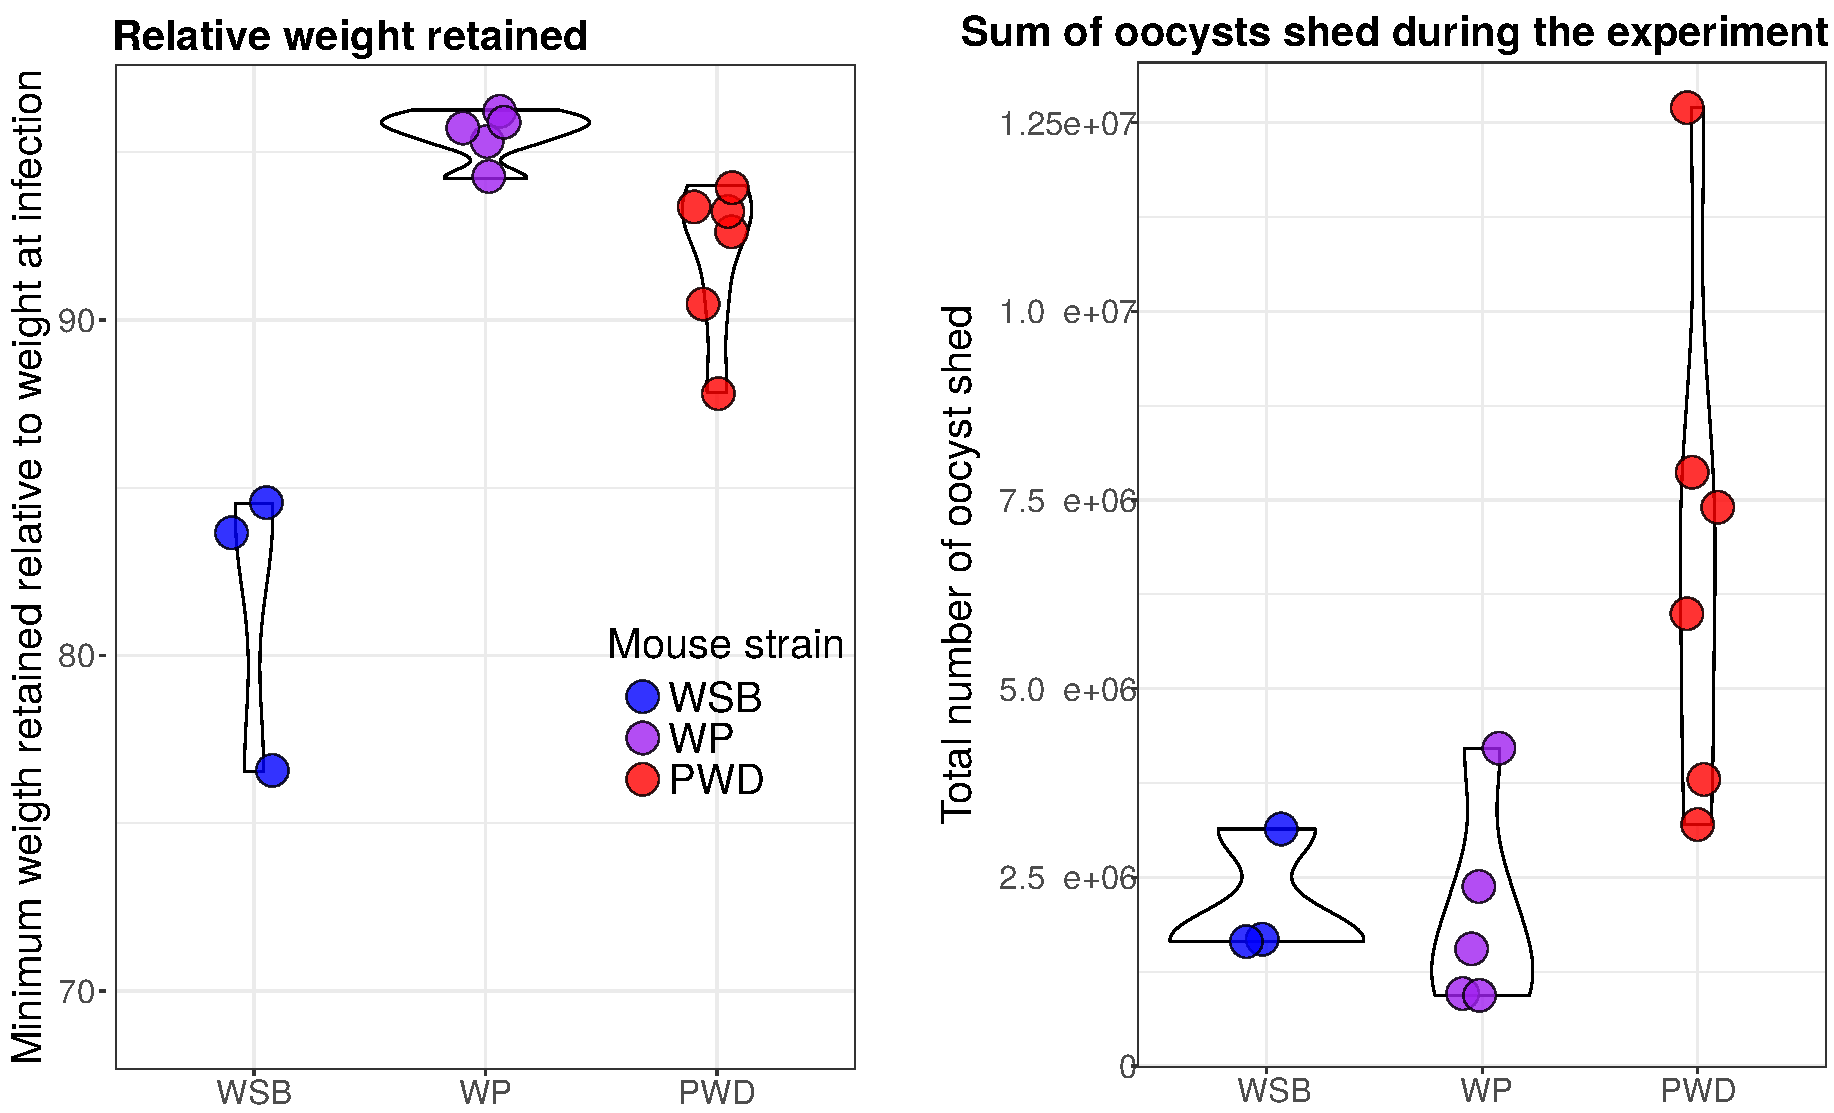
\includegraphics[scale=1.1]{May2017_E64.pdf}

  \end{center}
  
  some stats here!
  OUR MODEL +lm
}

\block{Perspective}
{
  \begin{center}
  \begin{itemize}
        \item Next cross infection experiment : verify our hypotheses (hybrid vigor, local adaptation), measure the effect of heterosis (within subspecies heterosis vs between subspecies)
        \item Assess local adaptation in other parasite strains
        \item Analyse of divergence scenarios for \textit{Eimeria} spp. based on whole genomes and comparison of models of coalescence and cospeciations with their murine hosts (beyond the house mouse).
        \item Investigation of loci of coevolution, identifying parasite genes under divergent selection in the two house mouse subspecies. The coevolving loci corresponding on the host side will be investigated.
  \end{itemize}

  \end{center}
}

% REFERENCES
% ----------

\block{References}
      {
        \begin{small}
          
          \hangindent=2cm Baird \textit{et al.} (2012) Where Are the Wormy Mice? A Reexamination of Hybrid Parasitism in the European House Mouse Hybrid Zone
           \textit{Evolution} 66 (9): 2757--72

          \hangindent=2cm Jost (2016) Improvement of Genetic Markers and Phylogenetics of Eimeria Spp. from House Mouse
          Edited by Emanuel Heitlinger. \textit{Humboldt University}

          \hangindent=2cm Heitlinger \textit{et al.} (2014) The genome of Eimeria falciformis-reduction and specialization in a single host apicomplexan         parasite.\\ \textit{BMC genomics} 15 (1), 696
                    
          \hangindent=2cm Machol\'{a}n \textit{et al.} (2012) Evolution of the House Mouse
          \textit{Cambridge University Press}
          
        
          
        \end{small}
      }

\end{columns}

% ----------------
\end{document}
\endinput
%%
%% End of file 
